\chapter{Aportaciones}

\section{Planificación}

Para el desarrollo de este proyecto, se ha requerido llevar a cabo una serie de tareas con diferentes dificultades e importancias. A continuación, se muestra una planificación general del mismo en la tabla \ref{tabla_planificación}, junto con las fases que componen su desarrollo, y una planificación temporal de cada apartado por separado,  (para obtener información adicional, véase el apéndice \ref{planificacion}). Cabe destacar que, cada apartado, se basa en los conocimientos adquiridos en los apartados anteriores, a la vez que introduce conceptos nuevos y mejora las prestaciones del modelo. De esta manera, cada apartado supondrá retos nuevos nunca antes vistos y, si un apartado anterior presenta algún fallo desconocido en el momento, se deberá volver a la etapa anterior y subsanarlo. Tras solventarlo, se podrá proseguir con la etapa posterior. Además, dada la naturaleza de `caja negra' de las redes neuronales, estas presentan cierta dificultad a la hora de depurar el código. Por tanto, esto supondrá un tiempo de depuración considerable en todas y cada una de las implementaciones, tal y como se mostrará a continuación.

\begin{enumerate}[label=\textbullet]
	\item \textbf{Estudio previo}: Consiste en el estudio y comprensión de cuestiones generales, dentro del campo de aprendizaje automático y visión por computador, comunes a redes neuronales totalmente conectadas, y redes neuronales convolucionales.
	
	\item \textbf{Investigación y desarrollo de redes neuronales totalmente conectadas}: En este periodo, me centré en la investigación y comprensión sobre las redes neuronales totalmente conectadas a bajo nivel. De esta manera, sabía que podría generar cualquier tipo de red totalmente conectada de manera dinámica, sin necesidad de realizar ningún tipo de cálculo posterior, independientemente del lenguaje de programación empleado, así como del uso o no de librerías que faciliten el proceso. 
	
	\item \textbf{Investigación y desarrollo de redes neuronales convolucionales}:
	Una vez familiarizado con redes neuronales totalmente conectadas, se trató de comprender de igual forma las redes neuronales convolucionales, pues se encuentran ampliamente relacionadas.
	\item \textbf{Investigación y desarrollo de sistemas homogéneos con OpenMP}:
	
	Una vez, comprendido el funcionamiento tanto de las redes neuronales totalmente conectadas, como de las redes neuronales convolucionales, me centré en reducir los tiempos de cómputo requeridos en ellas, mediante un paralelismo orientado a datos con OpenMP, (se analizará en detalle en secciones posteriores).
	
	\item \textbf{Investigación y desarrollo de sistemas heterogéneos con CUDA y cuDNN}:
	Con el conocimiento teórico y práctico ya adquirido sobre sistemas homogéneos, aplicados tanto a redes neuronales totalmente conectadas como a redes neuronales convolucionales, se avanza ahora hacia la exploración de sistemas heterogéneos, aplicados a estas mismas arquitecturas de redes neuronales.
\end{enumerate}


\begin{table}[H]
	\centering
	\begin{tabular}{|lll|}
		\hline
		Apartado 	 &\vline  & Tiempo (Horas) \\
		\hline
		
		Estudio previo    & \vline & 16 \\			
		\hline
		Investigación y desarrollo  	 & \vline & 	\\
		de redes neuronales  	 & \vline & 143	\\
		totalmente conectadas 	 & \vline & 	\\
		\hline
		Investigación y desarrollo    & \vline & 	 \\	
		de redes neuronales    & \vline & 152	 \\			
		convolucionales    & \vline & 	 \\					
		\hline
		Investigación y desarrollo  	 & \vline & 	 \\
		de sistemas homogéneos  	 & \vline & 103	 \\
		con OpenMP 	 & \vline & 	 \\
		\hline
		Investigación y desarrollo     & \vline &  	\\
		de sistemas heterogéneos    & \vline &  \\ 
		con CUDA y cuDNN    & \vline & 282 \\ 	
		\hline
		\hline
		Tiempo total:				& \vline & 696 \\
		\hline
	\end{tabular}
	\caption{Planificación del proyecto}
	\label{tabla_planificación}
\end{table}


\section{Paralelización mediante OpenMP}

\subsubsection{Tipos de paralelismo}

El entrenamiento de una red neuronal convolucional (CNN) se puede paralelizar de diversas maneras. Cuando el modelo se divide entre varios ordenadores que son entrenados con los mismos datos, se conoce \textbf{paralelismo del modelo} \cite{data_model_parallelism} (por ejemplo, asignando una capa por computador). Por otro lado, cuando se distribuyen los datos entre múltiples nodos, pero se utiliza el mismo modelo para el entrenamiento en cada uno de ellos, se denomina \textbf{paralelismo de datos} \cite{model_parallelism}. En este proyecto, la implementación con OpenMP se basará en un paralelismo de datos, mientras que las implementaciones heterogéneas, utilizando CUDA y cuDNN, se fundamentarán en el paralelismo del modelo. \\

\subsubsection{Paralelismo en SGD con OpenMP}
\begin{algorithm}[H]
	\caption{Descenso del gradiente estocástico} 
	\begin{algorithmic}
		\State Datos de entrenamiento $D=\{(x_1, y_1), (x_2, y_2), ..., (x_N, y_N)\}$.
		
		\For{cada trabajador $t =0, ..., T-1$ en paralelo}
		\For{época $p\in\{0, ..., P-1\}$}
			\State Desordenar vector de datos D.
				\For{cada mini batch $m =0, ..., M-1$}
					\State Inicializar $gradientes^t$ a 0.
					\State Reparto de datos del batch m al trabajador t
					\State Realizar propagación hacia delante
					\State Obtener error total con la función de pérdida
					\State Cada trabajador t realiza la propagación hacia 
					\State detrás y obtiene el gradiente con respecto a 
					\State cada parámetro del modelo.
					
					\State Acumular gradientes obtenidos por cada trabajador t.
					\State Actualizar parámetros.
					
				\EndFor
			\EndFor
		\EndFor
	\end{algorithmic}
\end{algorithm}

La naturaleza iterativa del algoritmo del descenso del gradiente estocástico, podría parecer un impedimento para la paralelización del entrenamiento del modelo, ya que, la iteración \textit{i}, depende del resultado obtenido en la iteración \textit{i-1}. Sin embargo, tal y como se expone en \cite{CNN_parallel_Stanford}, \cite{CNN_parallel_International_Conference}, y \cite{CNN_parallel_Ome_Weird_Trick}, es posible implementar paralelismo en cada iteración del proceso. \\
En cada época el modelo, se entrena con \textit{M} subconjuntos de $N_m$ datos, los cuales son disjuntos entre sí. Dados \textit{T} ``trabajadores'' o procesos paralelos, cada subconjunto de $N_m$ datos (mini-batch), puede dividirse en \textit{T} subconjuntos de $\frac{N_m}{T}$ datos, asignando cada uno a un trabajador diferente.\\
De acuerdo con este enfoque, los datos de entrenamiento se distribuyen entre los distintos trabajadores \textit{T} tanto para la propagación hacia delante como para la retropropagación posterior. En el caso de la retropropagación, se debe acumular el gradiente de la pérdida con respecto a cada parámetro obtenido por cada trabajor. Una vez en posesión este gradiente `total', se procede a la actualización de los parámetros del modelo.

\begin{figure}[H]
	\centering
	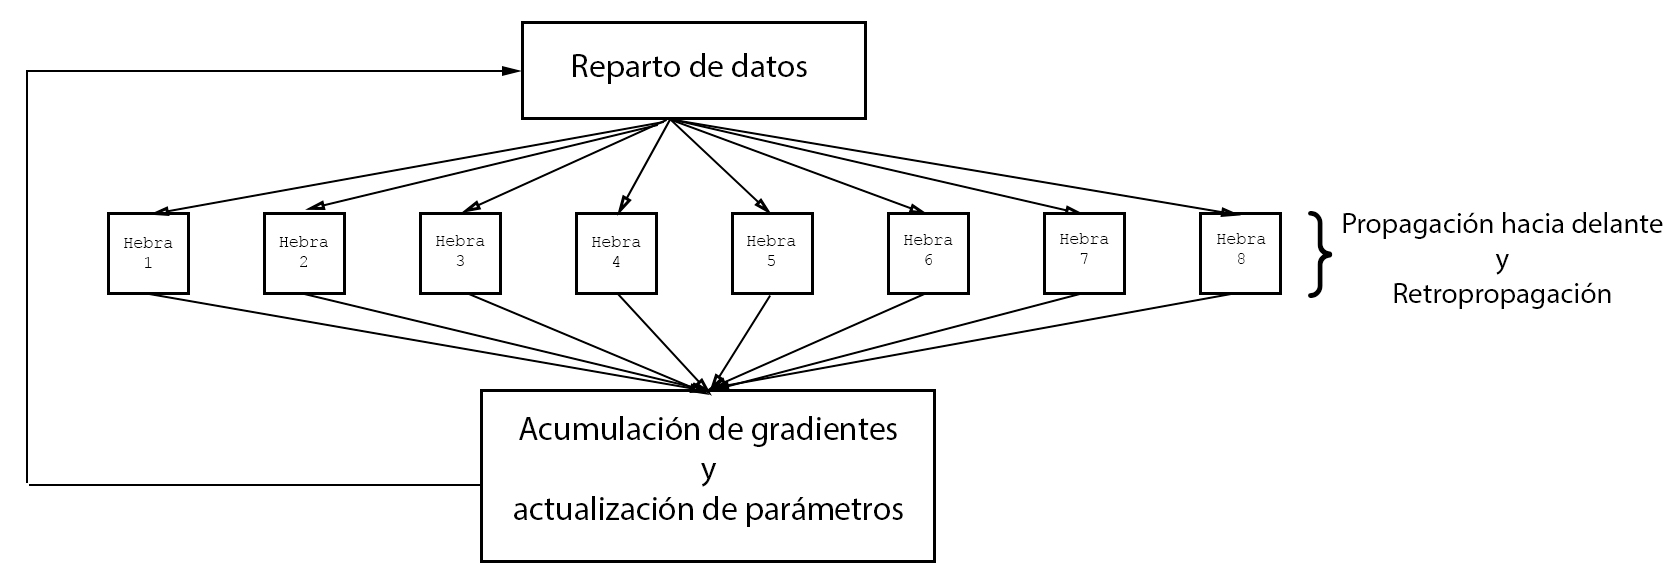
\includegraphics[width=1.2\linewidth]{imagenes/openmp_flujo.jpg} 
	\caption{Flujo de las hebras en la implementación con OpenMP}
	\label{fig:openmp_flujo}
\end{figure}

Tal como se muestra en la Figura \ref{fig:openmp_flujo}, aunque cada hebra realiza ciertas secciones de código en paralelo, como la propagación hacia delante o la retropropagación, existen momentos en los que estas hebras deben sincronizarse, como durante la distribución de los datos de un minibatch, o coordinarse para llevar a cabo operaciones conjuntas, como la acumulación y actualización de pesos.
